\documentclass{article}
\usepackage[utf8]{inputenc}
\usepackage{mathtext}
\usepackage{amsmath}
\usepackage[colorlinks=true, linkcolor=blue]{hyperref}
\usepackage[T1]{fontenc}
\usepackage[utf8]{inputenc}
\usepackage[english, bulgarian, russian]{babel}
\usepackage{tikz}
\usepackage{pgfplots}
\usepackage{indentfirst}
\usepackage[export]{adjustbox}
\usepackage{lipsum} % sample text
\usepackage{floatflt}
\usepackage{multirow}
\usepackage{geometry} 
\usepackage{animate}
\geometry{verbose,a4paper,tmargin=2cm,bmargin=2cm,lmargin=1.5cm,rmargin=1.5cm}
\setlength{\parindent}{0.65cm}
\setlength{\parskip}{0.15cm}

\usepackage{wrapfig}
\usepackage{array,graphicx,caption}


%Матеша
\usepackage{amsmath,amsfonts,amssymb,amsthm,mathtools} % AMS
\usepackage{icomma} % "Умная" запятая

%\mathtoolsset{showonlyrefs=true} % Показывать номера только у тех формул, на которые есть \eqref{} в тексте.

%% Шрифты
\usepackage{euscript}	 % Шрифт Евклид
\usepackage{mathrsfs} % Красивый матшрифт

%% Свои команды
\DeclareMathOperator{\sgn}{\mathop{sgn}}

%% Перенос знаков в формулах (по Львовскому)
\newcommand*{\hm}[1]{#1\nobreak\discretionary{}
	{\hbox{$\mathsurround=0pt #1$}}{}}
\begin{document}

 
\begin{titlepage}
     \begin{center}
     \large Московский физико-технический институт\\
    (национальный исследовательский университет)\\
    \vspace{4cm}
    \Large Лабораторная работа № 5.5.5 по курсу \\  Квантовая физика\\
    \vspace{4cm}
    \textbf{\Huge <<Компьютерная сцинтилляционная \\ $\gamma$ - спектрометрия>>}\\
     \end{center}
    \vspace{5cm}
    {\par \raggedleft \large Выполнили:\\ студентки 3 курса
    103 группы\\Фитэль Алена\\ Флоренская Лидия \par}
    \vspace{3cm}
    \begin{center}
        Москва, 05.12.23 г
    \end{center}
\end{titlepage}

\section{Теоретическое введение}

\subsection*{Процессы взаимодействия гамма-излучения с веществом}
Основными процессами взаимодействия гамма-излучения с веществом являются:
\begin{enumerate}
    \item Фотоэффект - процесс взаимодейтвия гамма-кванта с электроном, связанным с атомом, при котором электрону передается вся энергия гамма-кванта. 
    \begin{equation*}
        T_e = E_{\gamma} - I_i,
    \end{equation*}
    где $I_i$ - потенциал ионизации i-ой оболочки атома.
    \item Эффект Комптона - упругое рассеяние фотона на свободном электроне, совпровождающееся изменением длины волны фотона. Максимальная энергия образующихся комптоновских электронов соответствует рассеянию гамма-квантов на $ 2\pi $ и равна:
	
	\begin{equation}\label{E_compton}
	E_{с \_ max} = \dfrac{\hbar \omega}{1 + \dfrac{m_ec^2}{2\hbar\omega}}
	\end{equation}
 
    \item Процесс образования электрон-позитронных пар. Происходит при высокой энергии гамма-кванта. Появившийся в результате процесса образования пары элетрон теряет свою энергию на ионизацию среды. Позитрон будет двигатся до тех пор, пока практически не остановится, аннигилирует с элетроном среды, в результате чего появятся два гамма-кванта. Далее возможны три варианта:
    \begin{enumerate}
        \item оба родившихся гамма-кванта не вылетают из детектора, и тогда вся энергия первичного гамма-кванта останется в детекторе, а в спектре появится пик с $E = E_{\gamma}$;
        \item один из родившихся гамма-квантов покидает детектор, и в спектре появляется пик, соответствующий энергии $E = E_{\gamma} - E_0$ , где $Е_0 = mc^2 =511~ кэВ$;
        \item  оба родившихся гамма-кванта покидают детектор, и в спектре появляется пик, соответствующий энергии $E = E_{\gamma} - 2E_0$;
    \end{enumerate}
\end{enumerate}
Помимо этих процессов  взаимодействия гамма-излучения с веществом, добавляются экспонента, связанная с наличием фона, пик характеристического излучения, возникающий при взаимодействии гамма-квантов с окружающим веществом, а также пик обратного рассеяния, образующийся при энергии квантов $ Е_\gamma \gg mc^22/2 $ в результате рассеяния гамма-квантов на большие углы на материалах конструктивных элементов детектора и защиты. Положение пика обратного рассеяния определяется по формуле ($ E $ --- энергия фотопика):
	
	\begin{equation}\label{Eobr}
		E_{обр} = \dfrac{E}{1 + \dfrac{2E}{mc^2}}
	\end{equation}

\subsection*{Энергетическое разрешение спектрометра }
%	
	Энергетическим разрешением спектрометра называется величина
	
	\begin{equation}\label{Ri = dE/E}
	R_i = \dfrac{\Delta E_i}{E_i}
	\end{equation}
	
	т.е. отношение ширины пика полного поглощения (измеренной на полувысоте) к регистрируемой энергии пика поглощения. Это значение $ E_i \propto \overline{n_i} $ --- числу частиц на выходе ФЭУ. При этом  $ \Delta E_i \propto \overline{\Delta n_i} = \sqrt{\overline{n_i}} $ --- ширина пика пропорциональна среднеквадратичной флуктуации, которая равна корню из числа частиц. Таким образом, наша формула \eqref{Ri = dE/E} примет вид
	
	\begin{equation}\label{Ri = c/E}
	R_i = \dfrac{\mathrm{const}}{\sqrt{E_i}}
	\end{equation}

\newpage


\section{Экспериментальная установка}

\begin{wrapfigure}{r}{0.5\textwidth}
  \centering
  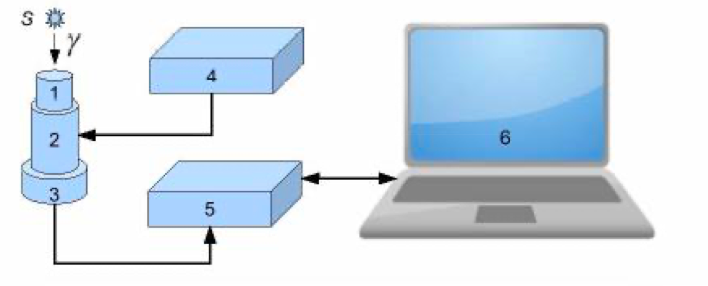
\includegraphics[width=0.48\textwidth]{Screenshot 2023-12-03 at 7.42.11 PM.png}
    
    \caption{Принципиальная блок-схема спектрометра. }
\label{schem}
  
  
\end{wrapfigure}
% Э\,к\,с\,п\,е\,р\,и\,м\,е\,н\,т\,а\,л\,ь\,н\,а\,я  \, у\,с\,т\,а\,н\,о\,в\,к\,а

Принципиальная блок-схема гамма-спектрометра
(\hyperref[schem]{Рисунок \ref*{schem}}):
\begin{enumerate}
    \item сцинтиллятор - кристалл NaI(Tl) с размерами 45$\times$50 мм и 20 $\times$ 25 мм, 
    \item фотоэлектронный умножитель (ФЭУ), 
    \item предусилитель импульсов, \item высоковольтный блок питания для ФЭУ, 
    \item блок преобразования аналоговых импульсов с ФЭУ в цифровой код (АЦП), 
    \item компьютер для сбора данных, их обработки и хранения.
\end{enumerate}




\section{Ход работы}

\subsection{Измерение значений фотопиков}
\begin{enumerate}

\item Снимем энергетические спектры с помощью экспериментальной установки для образцов $\mathrm{^{22}Na, \; ^{137}Cs, \; ^{60}Co, \; ^{241}Am}$ и $\mathrm{^{152}Eu}$ (см. \hyperref[prilosh]{Приложение}). По значениям каналов у пиков полного поглощения излучения от радиоактивных источников $^{60}Co, \; ^{137}Cs, \; ^{22}Na$ определим калибровочную формулу перехода от значений каналов к значениям энергий, используя табличные данные(\hyperref[table for E(N)]{Таблица \ref*{table for E(N)}}, \hyperref[calib]{Рисунок \ref*{calib}} ).

\begin{table}[h!]
        \centering
        \caption{Пики полного поглощения эталонных образцов}
        \begin{tabular}{|c|c|c|c|c|c|}
\hline
Элемент    & $^{60}Co$ & $^{60}Co$ & $^{137}Cs$ & $^{22}Na$ & $^{22}Na$ \\ \hline
$N_i$      & 1620      & 1840      & 960        & 750       & 1770      \\ \hline
$dN_i$     & 100       & 100       & 70         & 60        & 120       \\ \hline
$E_i$, МэВ & 1.173     & 1.332     & 0.662      & 0.511     & 1.274     \\ \hline
\end{tabular}
        \label{table for E(N)}
    \end{table}

\begin{equation}
        N = aE + b, \;\hspace{1 cm} a = 1.320 \pm 0.008 \;\frac{1}{\text{кэВ}},\hspace{1 cm} b = 83 \pm 9
\end{equation}

\item По полученной формуле посчитаем значения для пиков поглощения для различных материалов, а также ширину самих пиков - \hyperref[table all calc E(N)]{Таблица \ref*{table all calc E(N)}}.

\begin{table}[h!]
        
        \centering
        \caption{Пики полного поглощения исследуемых образцов}

\begin{tabular}{|l|l|l|l|l|l|}
\hline
Элемент    & $N_i$ & $\triangle N_i$ & $E_i$, МэВ & $\triangle E_i$, МэВ & $R_i$ \\ \hline
$^{22}$Na  & 750   & 60              & 510        & 50                   & 0.096 \\ \hline
$^{22}$Na  & 1770  & 120             & 1280       & 90                   & 0.073 \\ \hline
$^{60}$Co  & 1620  & 100             & 1160       & 80                   & 0.065 \\ \hline
$^{60}$Co  & 1840  & 100             & 1330       & 80                   & 0.059 \\ \hline
$^{137}$Cs & 640   & 120             & 420        & 90                   & 0.220 \\ \hline
$^{241}$Am & 110   & 20              & 20         & 20                   & 0.640 \\ \hline
$^{241}$Am & 160   & 20              & 61         & 15                   & 0.245 \\ \hline
$^{152}$Eu & 130   & 20              & 39         & 14                   & 0.355 \\ \hline
$^{152}$Eu & 250   & 30              & 120        & 20                   & 0.158 \\ \hline
$^{152}$Eu & 400   & 50              & 240        & 30                   & 0.141 \\ \hline
$^{152}$Eu & 530   & 50              & 340        & 40                   & 0.104 \\ \hline
\end{tabular}
        \label{table all calc E(N)}
    \end{table}


\begin{figure}[h!]
        \centering
        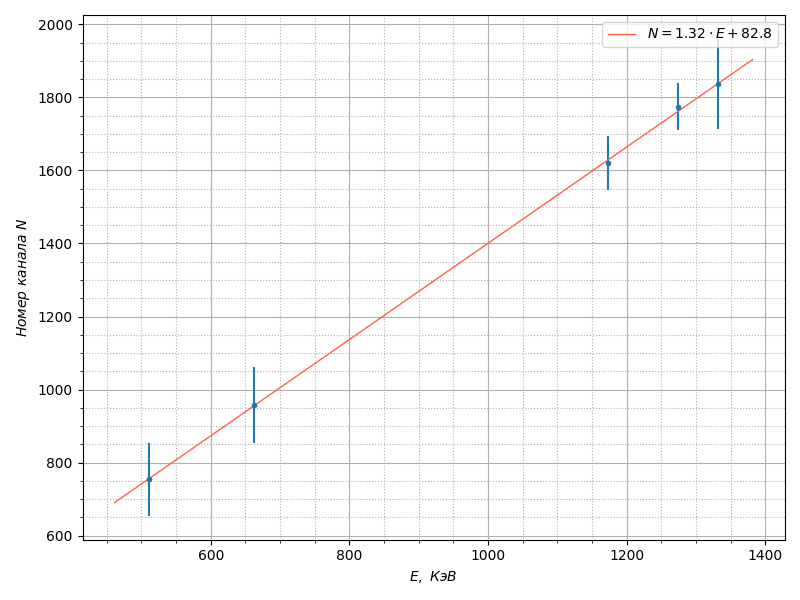
\includegraphics[width = 12 cm]{N(E).png}
        \caption{Калибровочная прямая N(E)}
        \label{calib}
    \end{figure}




\end{enumerate}








\subsection{Комптоновское рассеяние.}
Посмотрим на корреляцию значений края комптоновского рассеяния, полученных в ходе эксперимента, и  \hyperref[E_compton]{теоретического расчета} (\hyperref[E(E)]{Рисунок \ref*{E(E)}}, \hyperref[compton]{Таблица \ref*{compton}}). Получаем значение тангенста угла наклона линейной аппроксимации $k = 1.040 \pm 0.016 $. Таким образом, теоретический расчет близок к экспериментальным данным.

\begin{table}[h!]
\centering
\begin{tabular}{|l|r|r|l|l|l|}
\hline
Элемент & \multicolumn{1}{l|}{$N_e_d_g_e$} & \multicolumn{1}{l|}{$\triangle N_e_d_g_e$} & $E_e_d_g_e$, МэВ & $\triangle E_e_d_g_e$, МэВ & $E_e_d_g_e_t_h_e_o_r$, МэВ \\ \hline
$^{22}$Na  & 460  & 120 & 280 & 90  & 250 \\ \hline
$^{60}$Co  & 1220 & 260 & 860 & 190 & 810 \\ \hline
$^{137}$Cs & 640  & 120 & 420 & 90  & 370 \\ \hline
\end{tabular}
\caption{Значения пиков комптоновского рассеяния.}
\label{compton}
\end{table}



 \begin{figure}[h!]
        \centering
        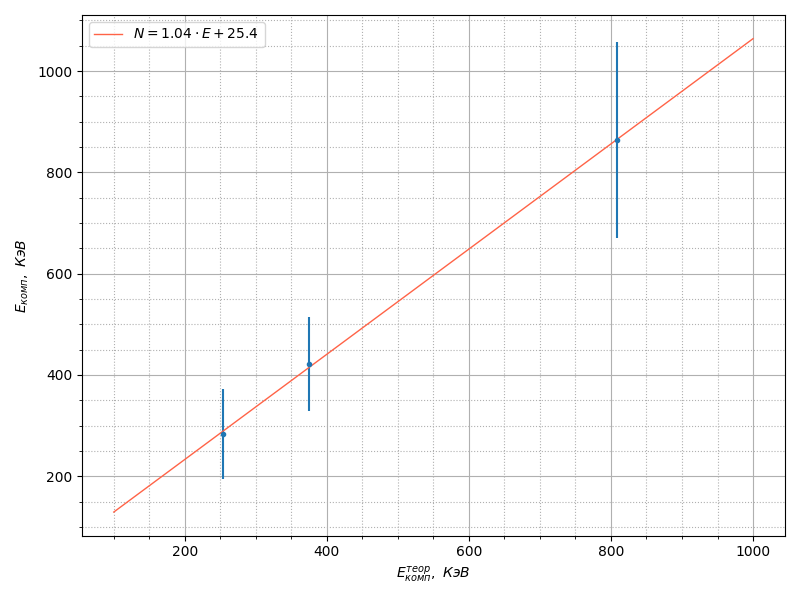
\includegraphics[width = 10 cm]{E(Etheor).png}
        \caption{График зависимости $E_{\text{комп}}(E_{\text{комп}}^{\text{теор}})$}
    \label{E(E)}
    \end{figure}

   %полностью сделано    
\subsection{Проверка формулы энергетического разрешения}

Построим график зависимости $R_i^2(1/E_i)$ (\hyperref[R2_and_invE]{Рисунок \ref*{R2_and_invE}}). Видно, что зависимость плохо описывается \hyperref[Ri = c/E]{линейной аппроксимацией}. 
    
\begin{figure}[h!]
        \centering
        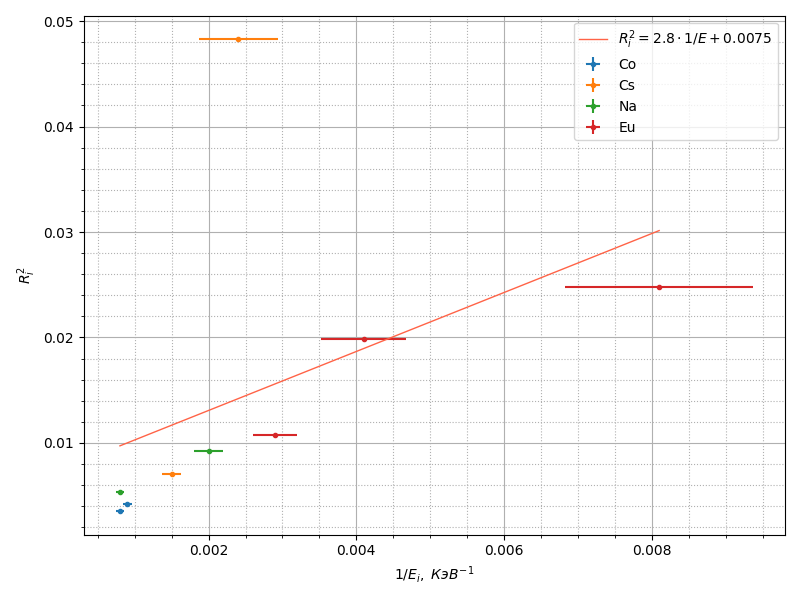
\includegraphics[width = 11 cm]{R(E).png}
        \caption{График зависимости $R_i^2(1/E_i)$}
        \label{R2_and_invE}
    \end{figure}
 
%полностью сделано
  %полностью сделано



  
\subsection{Обратное рассеяние}

Построим график зависимости $ E_{обр} = f(E)$ и нанесем экспериментальные точки(\hyperref[E_obr]{Рисунок \ref*{E_obr}}). В пределах погрешностей экспериментальные точки совпадают с  \hyperref[Eobr]{теоретически построенной зависимостью}. 


\begin{figure}[h!]
        \centering
        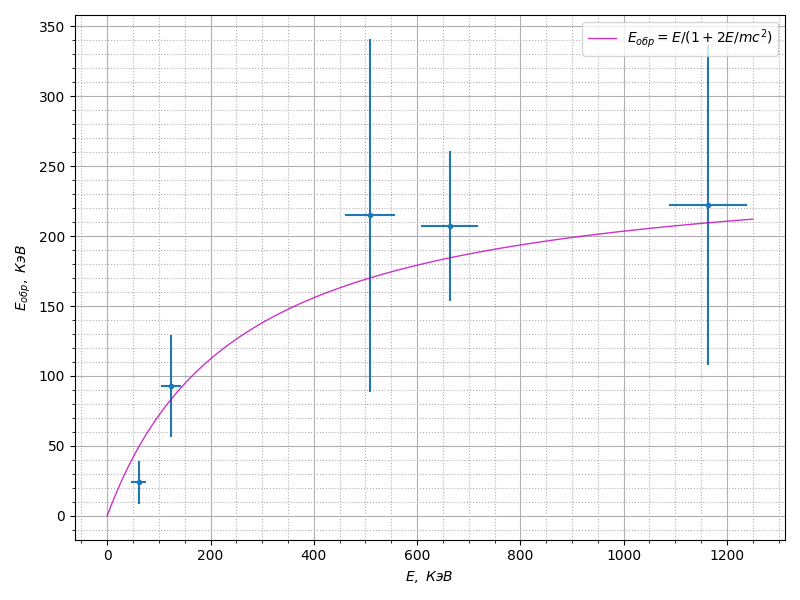
\includegraphics[width = 10 cm]{E(E).png}
        \caption{График зависимости $E_{\text{обр}}(E)$}
        \label{E_obr}
    \end{figure}




\subsection{Характеристическое излучение свинца}
Посмотрим на спектр фонового излучения (\hyperref[fone]{Рисунок \ref*{fone}}). На нем выделяется один пик, из аппроксимации гауссианом получим его значение: $E = 240 \pm 175 \text{ кэВ}$. 

\begin{figure}[h!]
        \centering
        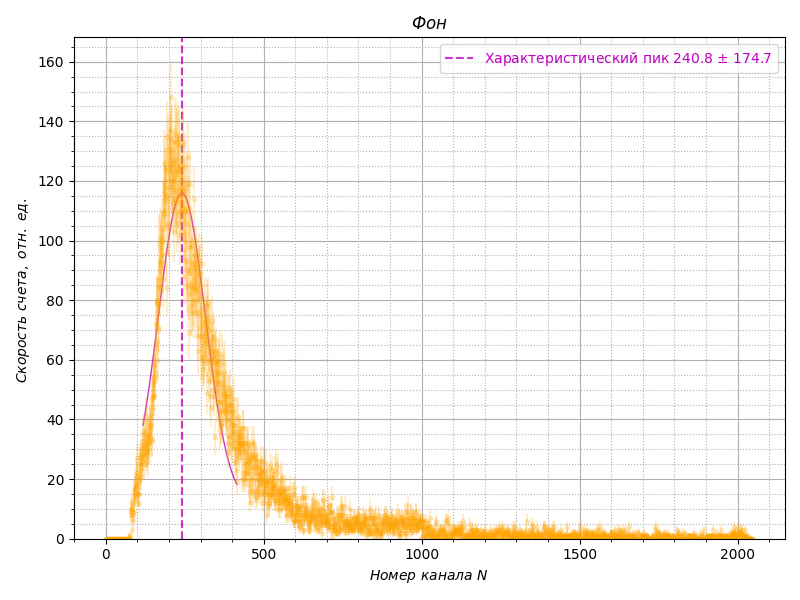
\includegraphics[width = 10 cm]{BBGG.png}
        \caption{Энергетический спектр фонового излучения}
        \label{fone}
    \end{figure}



\subsection{Оценка характеристик фотоэлектронного умножителя(ФЭУ)}
Осцилограмма импульсов на выходе ФЭУ имеет вид
    \begin{equation}
        U(t) = const \cdot e^{-\frac{t}{RC}} \left( 1 - e^{-\frac{t}{\tau_0}} \right),
    \end{equation}
    где $\tau_0$ -- время высвечивания сцинтиллятора, а $RC$ -- постоянная времени, $RC \gg \tau_0$.
По переденему фронту импульса можно оценить $\tau_0$:
    \begin{equation}
        U(t) \approx const \left( 1 - e^{-\frac{t}{\tau_0}} \right) \approx const \cdot \frac{t}{\tau_0}.
    \end{equation}

    Таким образом, $\tau_0$ можно оценить по прекращению нарастания импульса (т.е. на моменте, когда вырождается линейная зависимость): $\tau_0 = 1.8$ мкс. 

    По заднему фронту оценим $RC$, зафиксировав момент спада сигнала в $e$ раз: $RC = 5.2$ мкс.

\begin{figure}[h!]
        \centering
        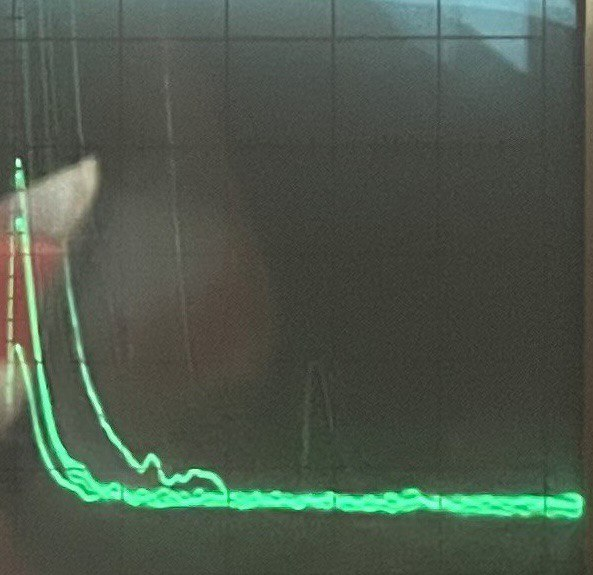
\includegraphics[width = 10 cm]{occct.jpg}
        \caption{Осцилограмма импульсов}
        \label{ooocccttt}
    \end{figure}










\section{Обсуждение результатов и вывод}

    В ходе работы были измерены спектры гамма-излучений для образцов $\mathrm{^{22}Na, \; ^{137}Cs, \; ^{60}Co, \; ^{241}Am}$ и $\mathrm{^{152}Eu}$, найдены для их пики полного поглощения, обратного рассеяния, а также комптоновские края. Проверены формулы для пиков обратного рассеяния и комптоновских краев.

    Найдено значение характеристического излучения свинца, служащего защитой спектрометра от внешнего излучения - $E = 240 \pm 175$.

    По форме импульсов на выходе ФЭУ оценены время высвечивания сцинтиллятора $\tau_0 = 1.8$ мкс, а также $RC = 5.2$ мкс -- постоянная времени цепи на выходе ФЭУ.


\newpage
\section*{Приложение} \label{prilosh}


Энергетические спектры образцов \hyperref[Na]{$\mathrm{^{22}Na$}}, \hyperref[Cs]{$\mathrm{^{137}Cs}$}, \hyperref[Co]{$\mathrm{^{60}Co}$}, \hyperref[Am]{$\mathrm{^{241}Am}$ }, \hyperref[Eu]{$\mathrm{^{152}Eu}$}:


\begin{figure}[h!]
        \centering
        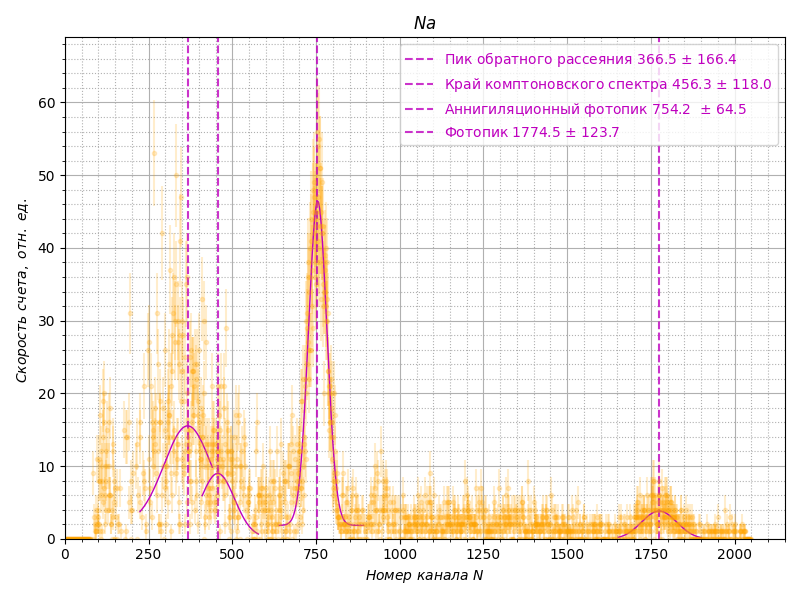
\includegraphics[width = 11 cm]{Nna.png}
        \caption{Энергетический спектр $\mathrm{^{22}Na}$}
        \label{Na}
    \end{figure}

\begin{figure}[h!]
        \centering
        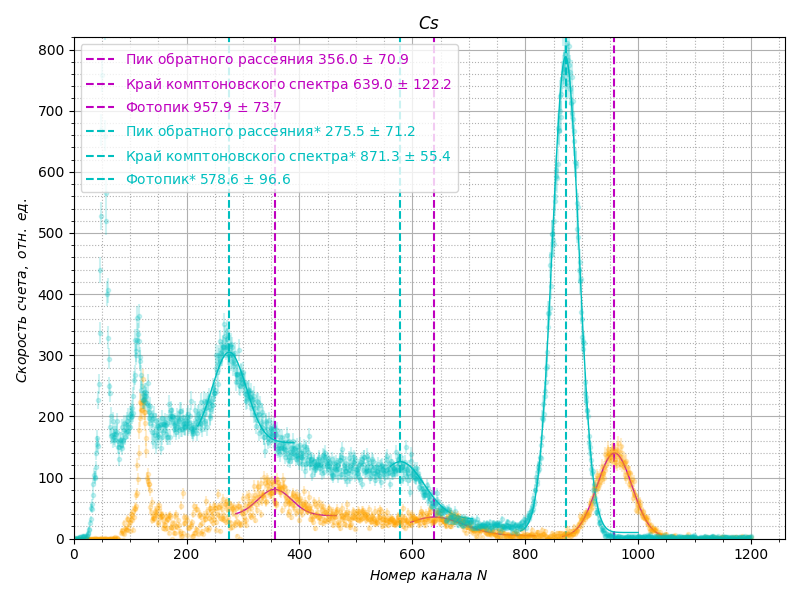
\includegraphics[width = 11 cm]{CSS.png}
        \caption{Энергетический спектр $\mathrm{^{137}Cs}$}
        \label{Cs}
    \end{figure}

\begin{figure}[h!]
        \centering
        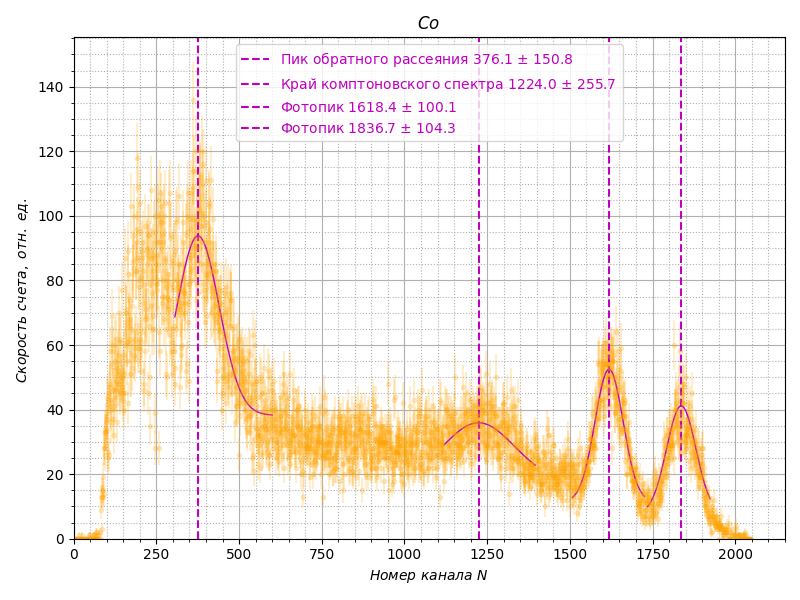
\includegraphics[width = 11 cm]{Cco.png}
        \caption{Энергетический спектр $\mathrm{^{60}Co} $}
        \label{Co}
    \end{figure}

\begin{figure}[h!]
        \centering
        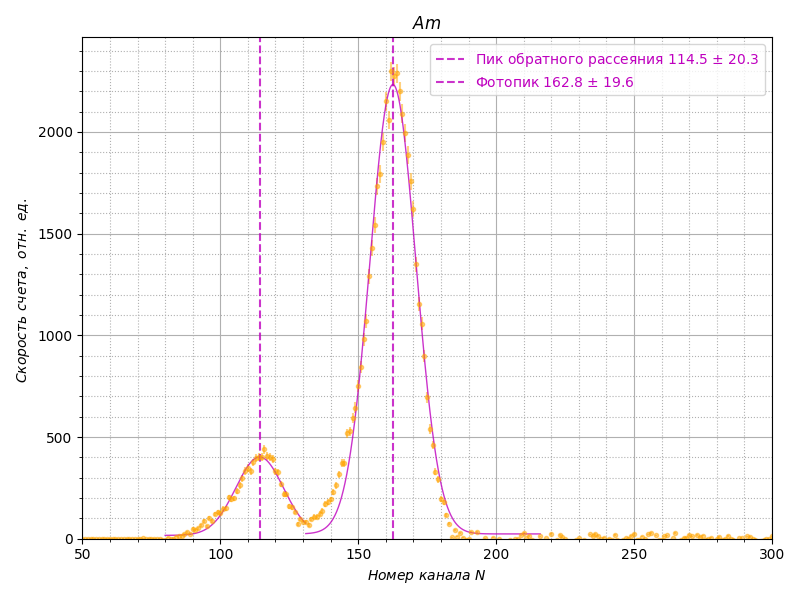
\includegraphics[width = 11 cm]{Aam.png}
        \caption{Энергетический спектр$\mathrm{^{241}Am} $}
        \label{Am}
    \end{figure}

\begin{figure}[h!]
        \centering
        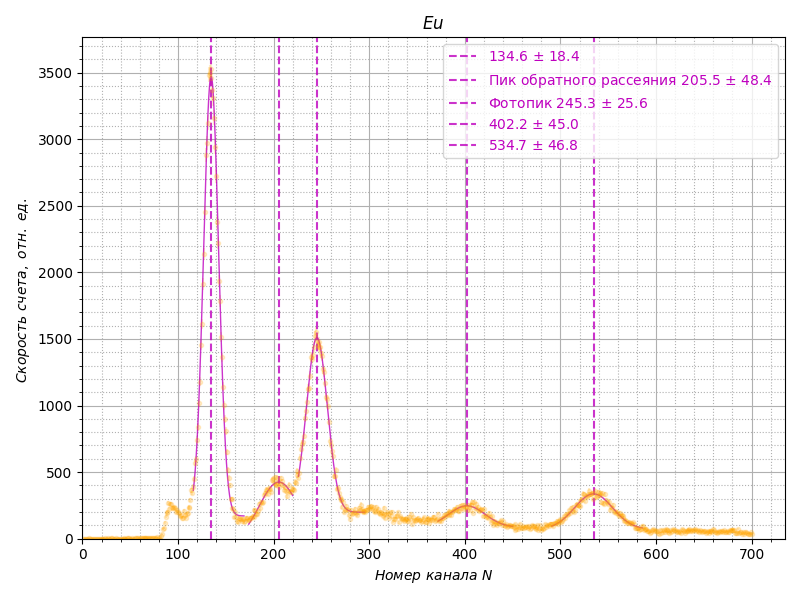
\includegraphics[width = 11 cm]{EEU.png}
        \caption{Энергетический спектр $\mathrm{^{152}Eu}$ }
        \label{Eu}
    \end{figure}




\end{document}
